%%%%%%%%%%%%%%%%%%%%%%%%%%%%%%%%%%%%%%%%%
% Stylish Article
% LaTeX Template
% Version 2.1 (1/10/15)
%
% This template has been downloaded from:
% http://www.LaTeXTemplates.com
%
% Original author:
% Mathias Legrand (legrand.mathias@gmail.com) 
% With extensive modifications by:
% Vel (vel@latextemplates.com)
%
% License:
% CC BY-NC-SA 3.0 (http://creativecommons.org/licenses/by-nc-sa/3.0/)
%
%%%%%%%%%%%%%%%%%%%%%%%%%%%%%%%%%%%%%%%%%

%----------------------------------------------------------------------------------------
%	PACKAGES AND OTHER DOCUMENT CONFIGURATIONS
%----------------------------------------------------------------------------------------

\documentclass[fleqn,10pt]{SelfArx} % Document font size and equations flushed left

\usepackage[english]{babel} % Specify a different language here - english by default

\usepackage{lipsum} % Required to insert dummy text. To be removed otherwise
\usepackage[bookmarks=true,pdfborder={0 0 0}]{hyperref}
\hypersetup{colorlinks=TRUE,linkbordercolor=red,linkcolor=green,pdfborderstyle={/S/U/W 1}}
\usepackage{amsmath} 
\usepackage{textcomp}



%----------------------------------------------------------------------------------------
%	COLUMNS
%----------------------------------------------------------------------------------------

\setlength{\columnsep}{0.55cm} % Distance between the two columns of text
\setlength{\fboxrule}{0.75pt} % Width of the border around the abstract

%----------------------------------------------------------------------------------------
%	COLORS
%----------------------------------------------------------------------------------------

\definecolor{color1}{RGB}{0,0,90} % Color of the article title and sections
\definecolor{color2}{RGB}{0,20,20} % Color of the boxes behind the abstract and headings

%----------------------------------------------------------------------------------------
%	HYPERLINKS
%----------------------------------------------------------------------------------------

\usepackage{hyperref} % Required for hyperlinks
\hypersetup{hidelinks,colorlinks,breaklinks=true,urlcolor=color2,citecolor=color1,linkcolor=color1,bookmarksopen=false,pdftitle={Title},pdfauthor={Author}}

%----------------------------------------------------------------------------------------
%	ARTICLE INFORMATION
%----------------------------------------------------------------------------------------

\JournalInfo{Data Mining B565 Fall 2016} % Journal information
\Archive{} % Additional notes (e.g. copyright, DOI, review/research article)

\PaperTitle{Advanced Regression Techniques : Housing Prices} % Article title

\Authors{Ankit Saxena\textsuperscript{1}*, Samvat Rastogi\textsuperscript{2},Shailendra Patil\textsuperscript{3}} % Authors
\affiliation{\textsuperscript{1}\textit{Data Science Science, School of Informatics and Computing, Indiana University, Bloomington, IN, USA}} % Author affiliation
\affiliation{\textsuperscript{2}\textit{ Data Science Science, School of Informatics and Computing, Indiana University, Bloomington, IN, USA}} % Author affiliation
\affiliation{\textsuperscript{3}\textit{ Data Science Science, School of Informatics and Computing, Indiana University, Bloomington, IN, USA}} % Author affiliation
\affiliation{*\textbf{Corresponding author}: samrasto@indiana.edu} % Corresponding author

\Keywords{Keyword1 --- Keyword2 --- Keyword3} % Keywords - if you don't want any simply remove all the text between the curly brackets
\newcommand{\keywordname}{Keywords} % Defines the keywords heading name

%----------------------------------------------------------------------------------------
%	ABSTRACT
%----------------------------------------------------------------------------------------

\Abstract{This project deals with predicting the Sales Price of individual residential properties in Ames, Iowa. The data set consists of both 'Training Data' and Test Data'. The goal is to fit an appropriate regression model using the 'Training Data' and then  predict the Sale Price for the given 'Test Data' based on the model. The 'Training Data' consist of 1460 observation and 81 Attributes including the Sales Price and 'Test Data' contains 1459 observations with 80 attributes which does not include Sales Price. Before applying any model, the data is preprocessed to take care of missing values and also to reduce number of attributes being used and then various regression methods like 'Linear', 'Random Forest' 'Gradient Boosting' , 'Xtreme Gradient Boosting' is applied and compared, and the model with least error rate is then used to predict the Sales Price for 'Test Data'. }

%----------------------------------------------------------------------------------------

\begin{document}

\flushbottom % Makes all text pages the same height

\maketitle % Print the title and abstract box

\tableofcontents % Print the contents section

\thispagestyle{empty} % Removes page numbering from the first page

%----------------------------------------------------------------------------------------
%	ARTICLE CONTENTS
%----------------------------------------------------------------------------------------

\section*{Introduction} % The \section*{} command stops section numbering
"The Housing Market refers to the supply and demand for houses, usually in a particular country or region. A key element of the housing market is the average house prices and trend in house prices"[1]. For many people buying a property is one of the important decisions in life. There are many factors, like Area, Neighbourhood, Connectivity, Transportation ,House Price etc that impacts this decision. 
Hence it becomes very important to know the trend in which the houses are being sold, so that as a buyer we might have a rough idea what can be the expected Price of a house.  The need for predictive analysis is what is required here. As a analyst , we build various model and predict the rough estimate of the prices, which then is used by the property evaluators for their clients.


\addcontentsline{toc}{section}{Introduction} % Adds this section to the table of contents


%------------------------------------------------

\section{Background}


%\begin{equation}
%\cos^3 \theta =\frac{1}{4}\cos\theta+\frac{3}{4}\cos 3\theta
%\label{eq:refname2}
%\end{equation}



\subsection{Data}
The data that has been provided for analysis consists of 3 files
\begin{enumerate}[noitemsep]
\item \textbf{train.csv}
\item \textbf{test.csv}
\item \textbf{data$\_$description.txt}
\end{enumerate}

Train and Test data files consists of a column named ID, which can be used to uniquely identify every house and 79 attributes that can be used to predict the Sale Price of the house. Train data file consists of an additional column named Sale Price. The Sale Price of the houses in the training data file can be used to build the model for prediction of the Sale Price of the Test data. The data$\_$description file provides all necessary information regarding the attributes.
The data was downloaded from 
\href{https://www.kaggle.com/c/house-prices-advanced-regression-techniques/data}{\color{blue}kaggle}.


\subsection{Data Description}
The training data has 79 attributes excluding the Sales Price and a total of 1460 values. The test data has 78 attributes and a total of 1459 values.
Data consists of \textbf{43 categorical attributes} and \textbf{36 numerical variables}. 
\\The \textbf{categorical variables} are: MSZoning, Street, Alley, LotShape, LandContour, Utilities, LotConfig, LandSlope, Neighborhood, Condition1, Condition2, BldgType, HouseStyle, RoofStyle, RoofMatl, Exterior1st, Exterior2nd, MasVnrType, ExterQual, ExterCond, Foundation, BsmtQual, BsmtCond, BsmtExposure, BsmtFinType1, BsmtFinType2, Heating, HeatingQC, CentralAir, Electrical, KitchenQual, Functional, FireplaceQu, GarageType, GarageFinish, GarageQual, GarageCond, PavedDrive, PoolQC, Fence, MiscFeature, SaleType
SaleCondition
\\The \textbf{numerical attributes} are: 
MSSubClass, LotFrontage, LotArea, OverallQual, OverallCond, YearBuilt, YearRemodAdd, MasVnrArea, BsmtFinSF1, BsmtFinSF2, BsmtUnfSF, TotalBsmtSF, X1stFlrSF, X2ndFlrSF, LowQualFinSF, GrLivArea, BsmtFullBath, BsmtHalfBath, FullBath, HalfBath, BedroomAbvGr, KitchenAbvGr, TotRmsAbvGrd, Fireplaces, GarageYrBlt, GarageCars, GarageArea, WoodDeckSF, OpenPorchSF, EnclosedPorch, X3SsnPorch, ScreenPorch, PoolArea, MiscVal, MoSold, YrSold




\subsection{Data Preprocessing}
The biggest task in any Data Mining problem is 'Data Preprocessing' . Before we apply any algorithms , we first need to clean the data. The data might contain missing values, outlier etc. There will be different kinds of attribute like continuous variables, categorical variables and so on. Such variables need to be taken care of based on the model we want to apply.  Data Preprocessing not only deals with these thing but also feature selection, data reduction etc. Given a set of attribute , not every attribute is important for data analysis or prediction, few attributes might be of no use and few attributes will be very vital for our analysis, so for this purpose we do Feature extraction. 
\subsubsection{Missing Data Imputation}
There are many attributes which have NA as one of the accepted value in their domain. These NA\textquotesingle s are not missing value but rather explain the absence of a particular feature in the house. The following attributes have NA in their domain:
Alley, BsmtQual, BsmtCond, BsmtExposure, BsmtFinType1, BsmtFinType2, FireplaceQu, GarageType, GarageFinish, GarageQual, GarageCond, PoolQC, Fence, MiscFeature.
The NA values for these attributes were replaced with \textbf{NC} while cleaning the data, to differentiate the actual missing values for other attributes with these 14 attributes.After replacing the NA values with NC for these attributes, we found the number of actual NA values or missing values:
A total of \textbf{357} values are missing in the Training data.
A total of \textbf{358} values are missing in the Test data.
The percentage of missing values in the training data is \textbf{0.3018\%}
The percentage of missing values in the test data is \textbf{0.3067\%}
\\ \\The majority of values are missing for the attribute \textbf{LotFrontage}
The percentage of missing values for LotFrontage in training data is \textbf{17.739\%}
The percentage of missing values for LotFrontage in test data is \textbf{15.558\%}
The mean of the values for attribute \textbf{LotFrontage} in training data is \textbf{70.05} and the median is \textbf{69.00}.
The mean of the values for attribute \textbf{LotFrontage} in test data is \textbf{68.58} and the median is \textbf{67.00}.
The missing values have been replaced with the mean of the existing values for LotFrontage, as there is not a huge difference between the mean and the median.
\\ \\The attribute \textbf{GarageYrBlt} has the second highest number of missing values.
The percentage of missing values for \textbf{GarageYrBlt} in training data is \textbf{5.547\%}
The percentage of missing values for \textbf{GarageYrBlt} in test data is \textbf{5.346\%}
The mean of the values for attribute \textbf{GarageYrBlt} in training data is \textbf{1979} and the median is \textbf{1980}.
The mean of the values for attribute \textbf{GarageYrBlt} in test data is \textbf{1978 }and the median is \textbf{1979}.
The missing values have been replaced with the mean of the existing values for GarageYrBlt, as there is not a huge difference between the mean and the median.
Similarly for all other numerical attributes missing values was replaced by Mean or Median based on data and for categorical attributes the missing values were replaced by the mode of that particular attribute.
%\begin{figure}[ht]\centering
%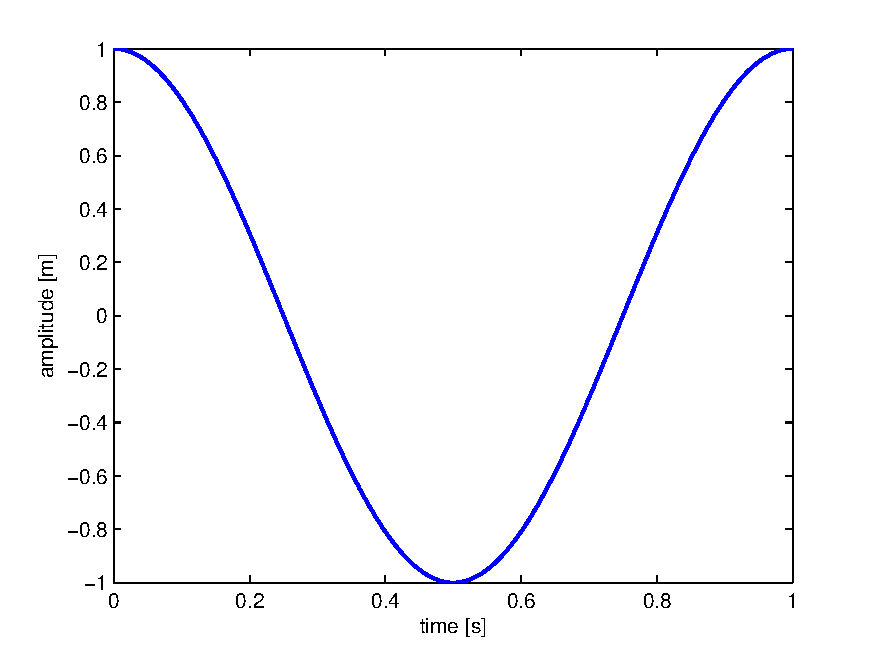
\includegraphics[width=\linewidth]{results}
%\caption{In-text Picture}
%\label{fig:results}
%\end{figure}
%
%Reference to Figure \ref{fig:results}.

%------------------------------------------------
\subsubsection{Feature Selection/Feature Selection}
\textbf{Feature extraction} starts from an initial set of measured data and builds derived values (features) intended to be informative and non-redundant, facilitating the subsequent learning and generalization steps, and in some cases leading to better human interpretations. Feature extraction is related to dimensionality reduction [5].
When the input data to an algorithm is too large to be processed and it is suspected to be redundant, then it can be transformed into a reduced set of features (also named a features vector). This process is called \textbf{feature selection} [5].
\\ \\One of the methods for data reduction is \textbf{Correlation}. Correlation is a statistical technique that can show whether and how strongly pairs of variables are related. 
\\ We are using \textbf{Pearsons Coeffiecient} and this can be done in \textbf{R} using \textbf{cor} function. Below is the graph that shows the correlation among all numerical attributes.
\begin{figure}[h]
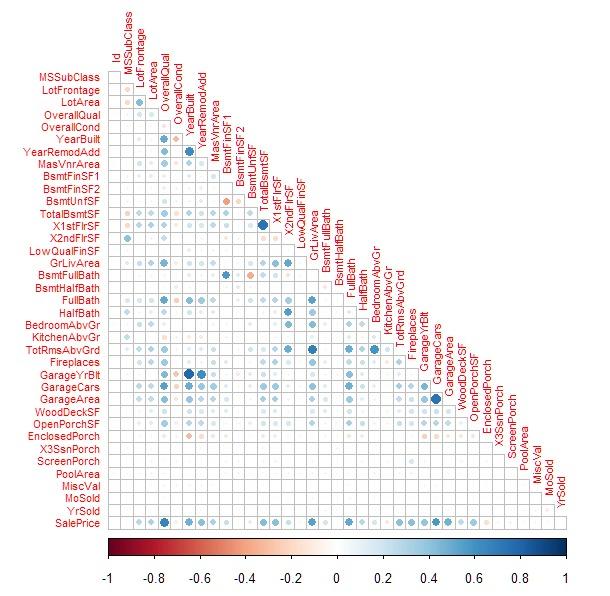
\includegraphics[scale=0.32]{Correlation}
\\ \caption{\\ Correlation Between Variables}
\end{figure}
As seen in the graph, the attributes OverallQual,GrLiveArea,FullBath, GarageCars are among few attributes which have greater correlation with SalePrice.
But the Pearson's cofficient needs linear data and data should be a normal, and as data size is small just by plotting the graphs its not easy to predict if the data is normal and attributes have linear relationship or not, hence correlation isn't a feasible idea here.
\\ \\ So the method we have used for feature extraction is using \textbf{Boruta Algorithm}. The algorithm is designed as a wrapper around a Random Forest classication algorithm. It iteratively removes the features which are proved by a statistical test to be less relevant than random probes. The \textbf{Boruta package} in \textbf{R} provides a convenient interface to the algorithm.
\\ \\Below is the step wise working of \textbf{boruta algorithm}[6]:
\begin{enumerate}[noitemsep]
\item Firstly, it adds randomness to the given data set by creating shuffled copies of all features (which are called shadow features).
\item Then, it trains a random forest classifier on the extended data set and applies a feature importance measure (the default is Mean Decrease Accuracy) to evaluate the importance of each feature where higher means more important.
\item At every iteration, it checks whether a real feature has a higher importance than the best of its shadow features (i.e. whether the feature has a higher Z score than the maximum Z score of its shadow features) and constantly removes features which are deemed highly unimportant.
\item Finally, the algorithm stops either when all features gets confirmed or rejected or it reaches a specified limit of random forest runs.
\end{enumerate}
The Boruta package was used after the missing values were replaced, as Boruta does not work if we have missing values in data.
After running the Boruta function and plotting the graph we get a list of \textbf{confirmed}, \textbf{tentative} and \textbf{rejected} attribute. Below is the graph of these variables
\begin{figure}[h]
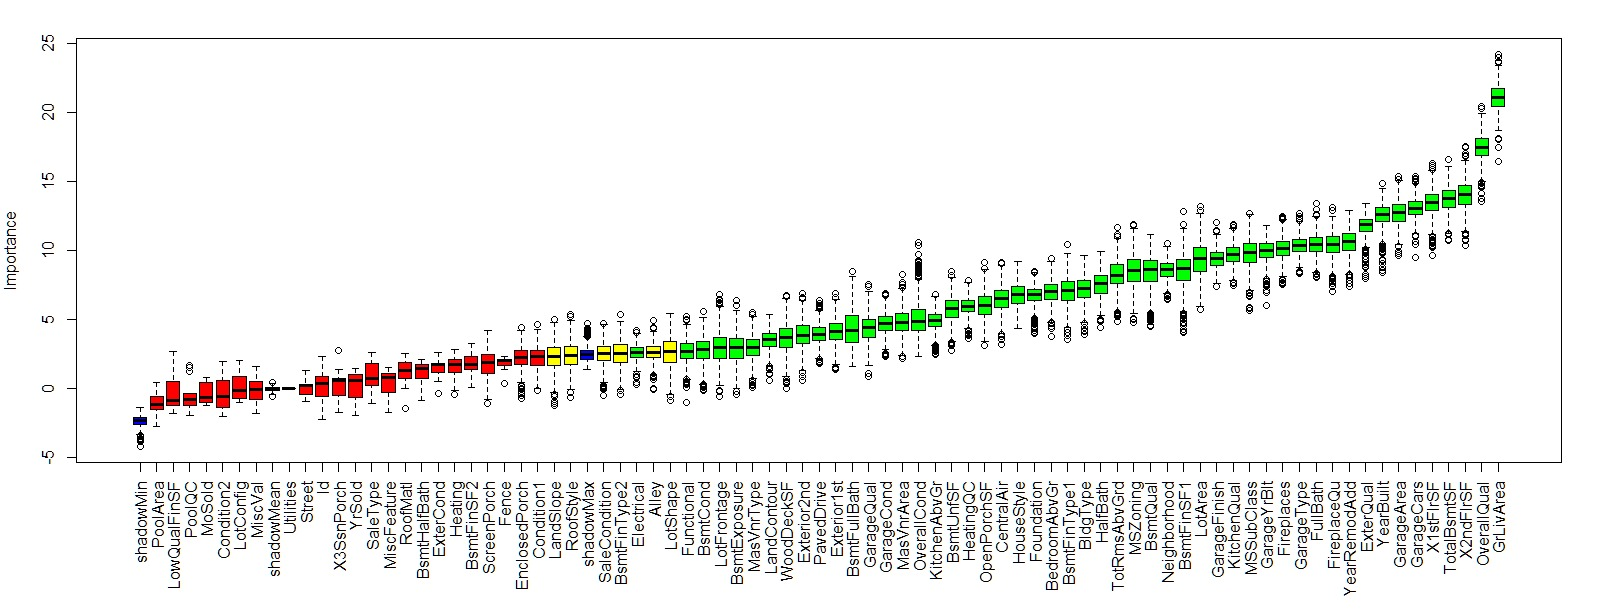
\includegraphics[scale=0.17]{Boruta}
\\ \caption{\\Boruta Plot}
\end{figure}
\\ The \textbf{green} box plots are for the attributes that have been confirmed, the \textbf{yellow} for tentative and \textbf{red} for rejected attributes.

\section{Algorithm and Methodology}
The project mainly deals with using various Regression techniques like \textbf{"Linear"},\textbf{"Random Forest Regression"},\textbf{"Gradient Boosting"},\textbf{"Extreme Gradient Boosting"} for predictive analysis.
\\ \textbf{What is Regression Analysis?}
\\Regression analysis is a form of predictive modelling technique which investigates the relationship between a dependent (target) and independent variable (s) (predictor). This technique is used for forecasting, time series modelling and finding the causal effect relationship between the variables [2]. 

\subsection{Regression Techniques}
\begin{enumerate}
\item \textbf{Linear Regression}
\newline A linear regression establishes a relation between a dependent variable (Y) and one or more independent variable(X) using a best fit straight line,(also known as "Regression Line").
\\ It is represented by below equation 
\begin{subequations}
\begin{align}
y & = a+bx 
\end{align}

%\begin{figure*}[!]% Using \begin{figure*} makes the figure take up the entire width of the page
%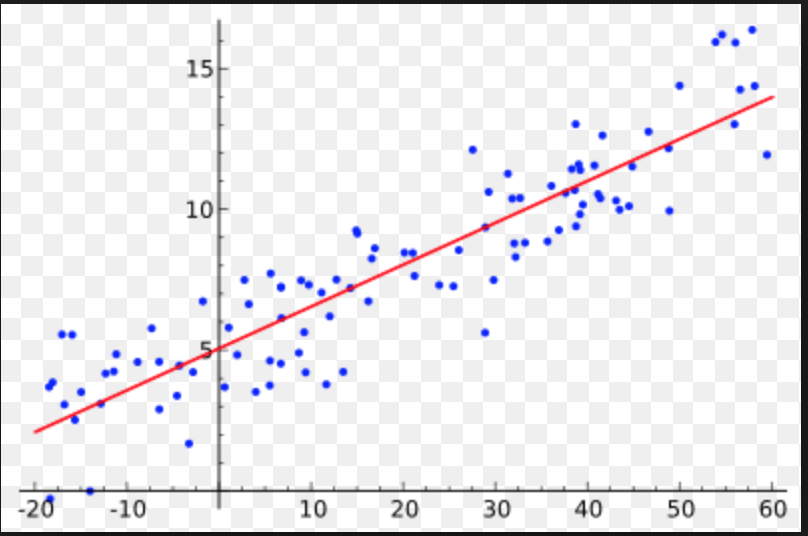
\includegraphics[scale=0.3]{Linearregression}
%\caption{Wide Picture}
%\label{fig:view}
%\end{figure*}

\begin{figure}[h]
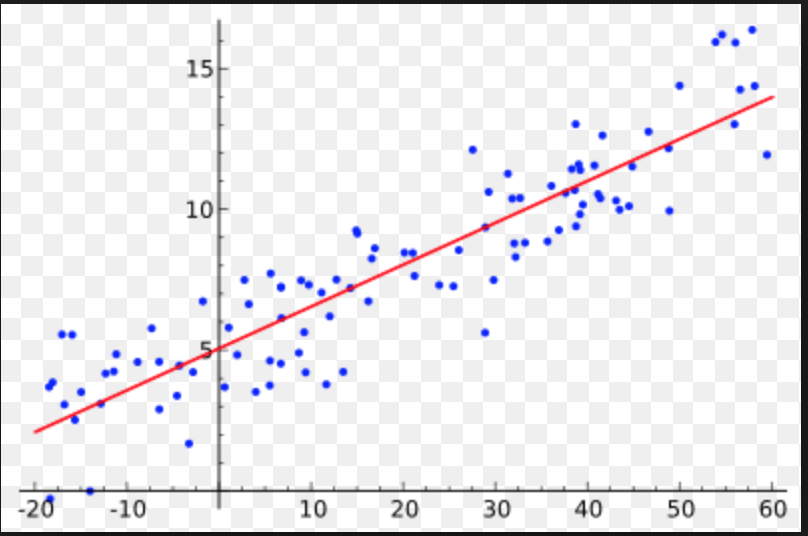
\includegraphics[scale=0.3]{Linearregression}
\\ \caption{\\ Linear Regression Line}
\end{figure}
\end{subequations}
\item \textbf{Random Forest Regression}
\\Random forests or random decision forests are an ensemble learning method for classification, regression and other tasks, that operate by constructing a multitude of decision trees at training time and outputting the class that is mean prediction (regression) of the individual trees [3].
\item \textbf{Gradient Boosting}
\\Gradient boosting is a machine learning technique for regression and classification problems, which produces a prediction model in the form of an ensemble of weak prediction models, typically decision trees. It builds the model in a stage-wise fashion like other boosting methods do, and it generalizes them by allowing optimization of an arbitrary differentiable loss function [4].
\item \textbf{LASSO Regression}:
lasso (least absolute shrinkage and selection operator) (also Lasso or LASSO) is a regression analysis method that performs both variable selection and regularization in order to enhance the prediction accuracy and interpretability of the statistical model it produces
\end{enumerate}
%\begin{table}[hbt]
%\caption{Table of Grades}
%\centering
%\begin{tabular}{llr}
%\toprule
%\multicolumn{2}{c}{Name} \\
%\cmidrule(r){1-2}
%First name & Last Name & Grade \\
%\midrule
%John & Doe & $7.5$ \\
%Richard & Miles & $2$ \\
%\bottomrule
%\end{tabular}
%\label{tab:label}
%\end{table}

\subsubsection{Subsubsection}

\lipsum[12] % Dummy text

\begin{description}
\item[Word] Definition
\item[Concept] Explanation
\item[Idea] Text
\end{description}

\subsubsection{Subsubsection}

\lipsum[13] % Dummy text

\begin{itemize}[noitemsep] % [noitemsep] removes whitespace between the items for a compact look
\item First item in a list
\item Second item in a list
\item Third item in a list
\end{itemize}

\subsubsection{Subsubsection}

\lipsum[14] % Dummy text

\subsection{Subsection}

\lipsum[15-23] % Dummy text

\section{Experiments and Results}

\section{Summary and Conclusions}
%------------------------------------------------
\phantomsection
\section*{Acknowledgments} % The \section*{} command stops section numbering

\addcontentsline{toc}{section}{Acknowledgments} % Adds this section to the table of contents

So long and thanks for all the fish \cite{Figueredo:2009dg}.

%----------------------------------------------------------------------------------------
%	REFERENCE LIST
%----------------------------------------------------------------------------------------
\phantomsection
[1]http://www.economicshelp.org/blog/glossary/definition-of-the-housing-market/
\newline [2]https://www.analyticsvidhya.com/blog/2015/08/comprehensive-guide-regression
\newline [3]https://en.wikipedia.org/wiki/Random$\_$Forest
\newline [4]https://en.wikipedia.org/wiki/Gradient$\_$boosting
\newline [5]https://en.wikipedia.org/wiki/Feature$\_$extraction
\newline [6]https://www.analyticsvidhya.com/blog/2016/03/select-important-variables-boruta-package/
\bibliographystyle{unsrt}
\bibliography{sample}

%----------------------------------------------------------------------------------------

\end{document}